% README.tex
% Based on File acl2012.tex
%
% Contact: Maggie Li (cswjli@comp.polyu.edu.hk), Michael White (mwhite@ling.osu.edu)
%%
%% Based on the style files for ACL2008 by Joakim Nivre and Noah Smith
%% and that of ACL2010 by Jing-Shin Chang and Philipp Koehn


%\usepackage{setspace}
%\doublespacing

\documentclass[11pt]{article}
\usepackage{latexsym}
\usepackage{amsmath}
\usepackage{multirow}
\usepackage{url}
\usepackage{pgfplots}
\usepackage{cite}
\makeatother
\usepackage[hidelinks]{hyperref}
\DeclareMathOperator*{\argmax}{arg\,max}
\pgfplotsset{compat=1.14}

\title{Optical Character Recognition through Convolutional Neural Networks}
\author{Jay Szeto\\ jsa143@sfu.ca \and Adrian Lim\\ aclim@sfu.ca}

\begin{document}

\maketitle

\begin{abstract}
      
\end{abstract}

\hrulefill

\section{Introduction}
    Optical Character Recognition (OCR) is the process of converting an image of text into computer readable text.\cite{ocr_wiki_2017} It can be used in applications such as data entry, license plate recognition, and defeating CAPTCHA anti-bot systems.\cite{ocr_wiki_2017} One approach for classification of characters involves the use of Convolutional Neural Networks (CNN).\cite{lecun_bottou_bengio_haffner_1998} This type of approach has grown more popular and complex in recent years which can be seen by the appearance of neural networks such as LeNet, ImageNet, and ResNet. \cite{lecun_bottou_bengio_haffner_1998, image_net_2012, he2016deep} Before character classification, text should be segmented into individual words or characters as incorrectly segmented text can cause improper classification. \cite{shinde_textpre-processing}
    
    In order to develop a deeper understanding of OCR using convoluted neural networks, we will be developing an OCR program that can read and classify characters in test images using the Tensorflow library. \cite{tensorflow15-whitepaper} These neural networks will be trained using font generated characters from the Char74k data set. \cite{deCampos09}
    
\section{Related Work}
    Aside just using a backpropagation algorithm, Tensorflow uses an assortment of other techniques/algorithms to enable proper training, such as softmax regression and stochastic gradient descent.
    
    Tensorflow provides a step-by-step tutorial on building a LeNet style CNN with dropout for classifying the MNIST data set.\cite{tensorflow15-whitepaper, lecun_bottou_bengio_haffner_1998} This provided a good starting point for applying a CNN to the Char74k data set.

\subsection{Softmax Regression}
Tensorflow uses the softmax regression function to generate the model for assigning probabilities.  This model uses two steps:
\begin{enumerate}
  \item Collect a sum of evidence values from input belonging to a certain class/label.
  \item Convert that evidence into probabilities.
\end{enumerate}
Evidence is gathered by performing a weighted sum of the pixel intensities.  A negative weight for a pixel represents evidence that is against the image being in that class (aka label).  Positive weights are treated as evidence in favor of labeling an image to said class.

Extra evidence, called bias, were also added.  These allow the algorithm to affect the evidence with weights "more likely independent of the input"~\cite{mnist-for-ml-beginners}.

Evidence for a class i given an input x is:
\begin{equation}
    evidence_{i} = \sum W_{i,j}x_{j} + b_{i}
\end{equation}


where $W_{i}$ is the weight and $b_{i}$ is the bias for class $i$, $j$ being an index allowing the summation of the pixels of the input image $x$.  
Once these evidences are available, a normalization of $e^x$ is required to calculate the necessary probabilities:
\begin{equation}
    softmax(evidence)_{i} = \frac{exp(x_{i})}{\sum exp(x_{j})}
\end{equation}

Exponentiation allows increases in evidence units to amplify our prediction probabilities, or simply the hypothesis, multiplicatively.  On the other hand, reduction in evidence amounts results in the hypothesis to reduce to a fraction of its original amount.

(The "Implementing the Regression" in first MNIST tutorial is after. However, the ItR section contains implementation details, proper placement of such info may be required...)


\subsection{Gradient Descent}




\section{Approach}
    - Note: ... (e.g. reader, cnn neural network layers.  one hot vectors (approach/research...?)from mnist for training, and later detecting features...)

    Note: intro to approach section here

\subsection{Pre-processing and Character Segmentation}
    
    In order to predict text from "real-life" images, the images will need to be segmented and normalized to reflect our training data. This was accomplished with a basic algorithm that first segmented the lines in the text and then segmented the characters in the text. Boxes around a test image where each line is found can be seen in figure \ref{fig:line_segmentation}. Boxes around each character found by the segmentation algorithm can be found in figure \ref{fig:character_segmentation}
    
    \begin{figure}
        \centering
        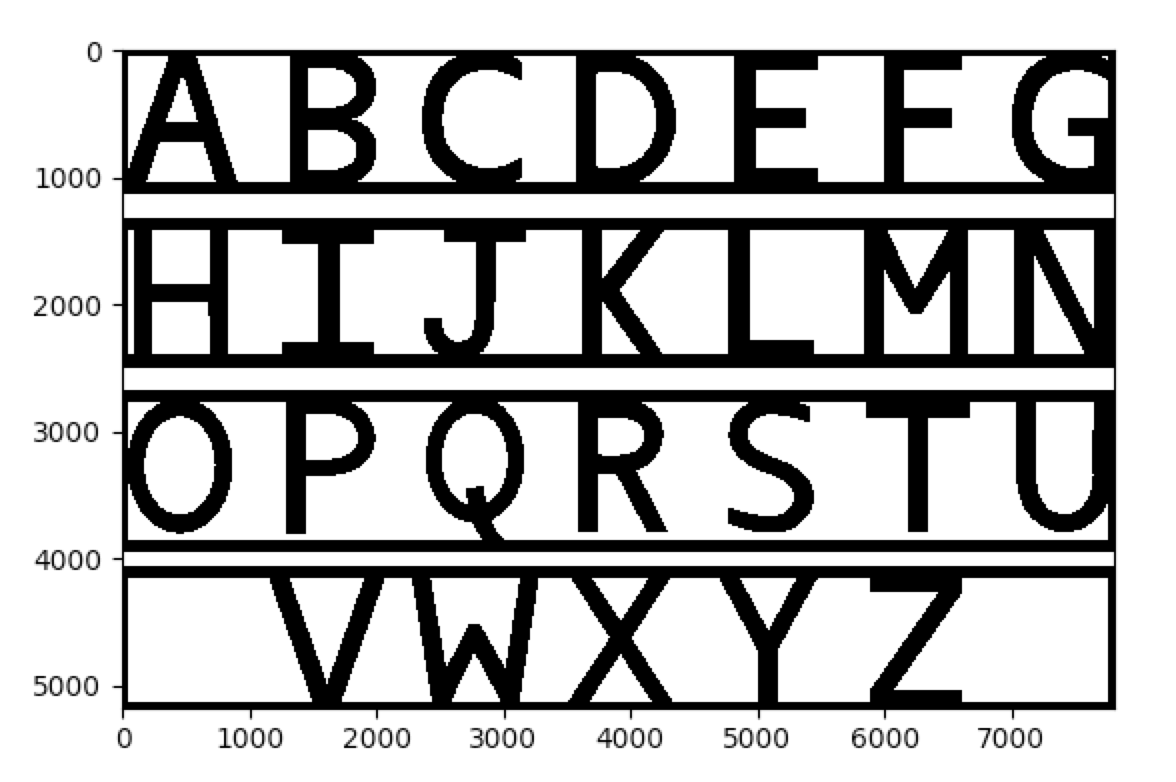
\includegraphics[scale=0.4]{line_segmentation_example.png}
        \caption{Line Detection and Segmentation}
        \label{fig:line_segmentation}
    \end{figure}
    
    \begin{figure}
        \centering
        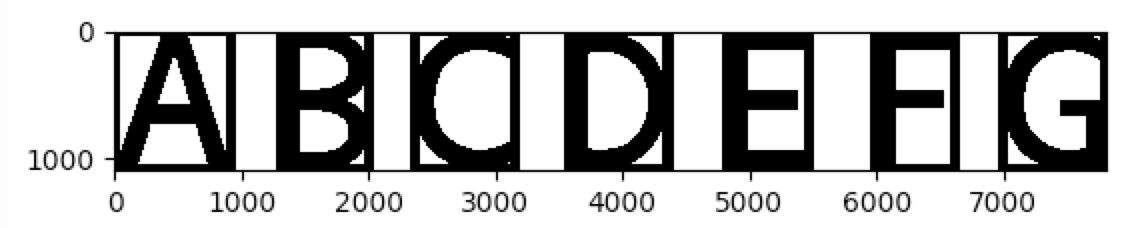
\includegraphics[scale=0.4]{character_segmentation_example.png}
        \caption{Character Detection and Segmentation}
        \label{fig:character_segmentation}
    \end{figure}

\subsection{Character Classification}

\subsubsection{The Architecture}
    To observe the effect of different parameters on the Convolutional Neural Network, we constructed multiple models.

    The first of our models was similar to the Tensorflow MNIST tutorial example except that we adjusted the final layer to output 62 different neurons as opposed to 10 to account for all of the classes of images in the Char74k data set.
    
    In our second model we added an additional convolutional layer and pooling layer and doubled the inital size of the input image.

-theorys/algorithms/procedures/concepts of neural networks

http://cs231n.github.io/convolutional-networks/

A letter classification process is used on the provided segmented image through multiple layers.  These layers consists three different types: convolutional, pooling, and dense layers. (Describe each layer here...)
\begin{enumerate}
  \item \textbf{Convolutional Layer:} A layer that applies convolution filters the input image with a ReLU activation function.  Each portion of the image will produce an individual value to the output map.
  \item \textbf{Max Pooling Layer:} extracts the data from convolutional layers to reduce the dimensions of the received feature map.  Due to the max pooling algorithm, only the maximum values will persist after such downsampling.  
  \item \textbf{Fully Connected Layer:} Unlike the convolutional and pooling layers, a fully connected layer receives and outputs a map of a constant size.
\end{enumerate}

(Describe structure of the CNN MNIST classifier)
\begin{enumerate}
  \item 
  \item 
  \item 
  \item 
  \item 
\end{enumerate}


The Tensorflow library was used to create/structure the neural network layers~\cite{tensorflow15-whitepaper}.


\subsubsection{Training}
https://www.tensorflow.org/get_started/mnist/beginners

The training of the convolutional neural network was implemented through the use of cross-entropy, backpropagation algorithm, and gradient descent optimization (caps?).



\begin{equation}
    y = softmax(evidence)    
\end{equation}

\begin{equation}
    softmax(x) = normalise(exp(x))
\end{equation}

\begin{equation}
    softmax(x) = \frac{exp(x_{i})}{\sum_{j} exp(x_{j})}
\end{equation}


\subsubsection{Predicting}

\section{Data}
The Chars74K's computer font dataset was used. This dataset contains 62992 "synthesised" characters~\cite{deCampos09}. They were chosen as the characters were centered in the middle of their images and the images were a constant size of 128 x 128.

\section{Results}
Directly results of our project (graphs and observations here)

\section{Discussion}


\section{Future Work}
Below are some brainstormed ideas for future work (Not exhaustive.  Section open to other ideas): 

- what can be improved 
    - e.g. character segmentation, 
    - ways to deal with noise, 
    - increasing number of layers...
    - etc
    
- what could we have done (if we had more time or resources...
    - e.g. specific details of how to char segmentation
    - noise dealing details
    - using specialized training images for specific
        reading situations
    
- how can we extend this further? What challenges will one might have to face?
    - e.g. algorithm to read documents...
    - text on meme reader
    - text on textbook reader (digital source)
    - text on a piece of paper (can easier be more noise)
        - but as similar in accuracy when reading from digital source, (suppose we read from high definition image of real textbook page to convert into digital source?
            - more issues if we make such a product since currently we assume text is parallel/horizontal
    




*Note: Future improvement, research showed that performing OCR (using...) is more effective in analyzing characters at the word level

*Note: lowercase letters same "size" as uppercase in dataset
http://yann.lecun.com/exdb/publis/pdf/lecun-01a.pdf



\section{Note to Self/Sources/References?(use bibliography instead of this section)}
Certain Tutorials were provided by Tensorflow regarding how to create our own MNIST Convolutional Neural Networks
\begin{verbatim}
https://www.tensorflow.org/get_started/mnist/mechanics
https://www.tensorflow.org/tutorials/layers
\end{verbatim}

\clearpage
\bibliography{project}
\bibliographystyle{ieeetr}

\end{document}

